\documentclass[10pt,letterpaper]{article}

\usepackage[utf8]{inputenc}
\usepackage[T1]{fontenc}
\usepackage{lmodern}
\usepackage[margin=0.45in,top=0.40in,bottom=0.40in]{geometry}
\usepackage{amsmath,amssymb,bm}
\usepackage{graphicx}
\usepackage{booktabs}
\usepackage{tabularx}
\usepackage{xcolor}
\usepackage{hyperref}
\usepackage[expansion=false]{microtype}
\usepackage{tcolorbox}
\usepackage{titlesec}
\usepackage{enumitem}

\graphicspath{{../figures/}{../../docs/engineering_reports/figures/}}

\definecolor{synspectivecrimson}{RGB}{140, 20, 40}
\definecolor{synspectivegold}{RGB}{205, 120, 20}
\definecolor{darkgray}{RGB}{35, 42, 54}
\definecolor{lightbg}{RGB}{253, 248, 249}
\definecolor{bordergray}{RGB}{235, 215, 220}

\hypersetup{
    colorlinks=true,
    linkcolor=synspectivecrimson,
    urlcolor=synspectivegold,
    citecolor=synspectivecrimson
}

\pagestyle{empty}

\titleformat{\section}{\large\bfseries\color{synspectivecrimson}}{}{0em}{}[\vspace{-0.4em}\rule{\linewidth}{0.8pt}\vspace{-0.3em}]

\tcbset{
    sharp corners,
    boxrule=0.8pt,
    colframe=synspectivecrimson,
    colback=lightbg,
    left=6pt,right=6pt,top=5pt,bottom=5pt
}

\begin{document}

% HEADER BOX
\begin{tcolorbox}[colframe=synspectivecrimson,colback=synspectivecrimson,coltext=white,boxrule=0pt,top=6pt,bottom=6pt]
\begin{minipage}[c]{0.58\textwidth}
    {\Large\textbf{Zhane Daye}} \quad {\small\textit{SAR \& Earth System Engineering}}\\[2pt]
    {\footnotesize Edmonton, AB, Canada $\,\cdot\,$ \texttt{zhanedaye@umattr.ca} $\,\cdot\,$ \href{https://www.linkedin.com/in/zhane-umattr}{linkedin.com/in/zhane-umattr}}
\end{minipage}
\hfill
\begin{minipage}[c]{0.40\textwidth}
    \raggedleft
    {\large\textbf{TARGET: SYNSPECTIVE}}\\[1pt]
    {\footnotesize\textbf{Role:} SAR Image Processing / InSAR Applied Scientist}\\[1pt]
    {\scriptsize StriX Constellation Land Displacement Monitoring (LDM)}
\end{minipage}
\end{tcolorbox}

\vspace{-4pt}

% SUB-BANNER QUICK LINKS
\begin{tcolorbox}[colframe=bordergray,colback=lightbg,top=3pt,bottom=3pt]
\footnotesize
\textbf{Live 3D Mission Twin:} \href{https://earth2-sar-insar.vercel.app#city=jp_tokyo&preset=sar_focus&stage=v3}{\texttt{earth2-sar-insar.vercel.app\#city=jp\_tokyo}} $\,\vert\,$ 
\textbf{Report (PDF):} \href{https://earth2-sar-insar.vercel.app/reports/EARTH2_X_BAND_SAR_INSAR_ENGINEERING_REPORT.pdf}{\texttt{SAR\_ENGINEERING\_REPORT.pdf}} $\,\vert\,$ 
\textbf{GitHub v1.0.0:} \href{https://github.com/zrt219/earth2studio/releases/tag/v1.0.0-mission-twin}{\texttt{v1.0.0-mission-twin}}
\end{tcolorbox}

\vspace{-4pt}

% TWO-COLUMN CORE CONTENT
\noindent
\begin{minipage}[t]{0.51\textwidth}
    \section*{The Operational Bottleneck}
    \footnotesize
    Synspective's StriX small-SAR constellation specializes in Land Displacement Monitoring (LDM) and disaster response. In steep mountainous regions like the Japanese Alps, severe typhoon landfall introduces two fatal radar signal degradations:
    \begin{enumerate}[leftmargin=12pt,topsep=1pt,itemsep=1pt,parsep=0pt]
        \item \textbf{Extreme Coherence Decay ($\gamma < 0.32$):} Intense precipitation saturates canopy and soil dielectric constants, triggering temporal and volumetric decorrelation that causes phase unwrapping to fail.
        \item \textbf{Layover \& Shadow Misattribution:} In steep slope terrain, ground subsidence can be indistinguishable from moisture-induced phase shifts without coupled atmospheric modeling.
    \end{enumerate}

    \section*{The Engineering Solution}
    \footnotesize
    I engineered a physical StriX-3 mission twin modeling descending passes ($561\text{ km}$ SSO, $34.1^\circ$ off-nadir) over Central Honshu during Typhoon Megi ($935\text{--}998\text{ hPa}$):
    \begin{itemize}[leftmargin=12pt,topsep=1pt,itemsep=1pt,parsep=0pt]
        \item \textbf{Repeat-Pass Coherence Loss Forward Modeling:} Formulated physical decay accounting for volumetric water convergence and slope gradients:
        \begin{equation*}
            \gamma_{\text{CCD}} = \gamma_0 \cdot \exp\left(-\alpha \cdot \Delta W_{\text{soil}} - \beta \cdot \|\nabla z_{\text{DEM}}\|\right)
        \end{equation*}
        Isolated \textbf{550.73 km$^2$} of high-risk mountain terrain ($\gamma < 0.32$, minimum $0.080$).
        \item \textbf{Autonomous STAC Tasking Triggers:} Hazard zones automatically generate OGC STAC v1.0.0 orders with full \texttt{sar:*} and \texttt{sat:*} metadata for StriX StripMap (VV/VH, 3m SLC).
        \item \textbf{Mesoscale InSAR APS Correction:} Evaluates Saastamoinen ZHD and Askne-Nordius ZWD across an $8\times$ upsampled grid ($0.03125^\circ \approx 3.4\text{ km}$), removing \textbf{9.24 atmospheric fringes} with a verified \textbf{98.81\% phase RMSE reduction} ($13.82\text{ rad} \rightarrow 0.16\text{ rad}$).
    \end{itemize}

    \section*{Verified Benchmark Record}
    \footnotesize
    \begin{tabularx}{\linewidth}{X r r}
        \toprule
        \textbf{Metric / Parameter} & \textbf{Raw InSAR} & \textbf{Engineered Twin} \\
        \midrule
        Honshu Severe Decorrelation & Unmapped & \textbf{550.73 km$^2$ ($\gamma < 0.32$)} \\
        Minimum Observed Coherence & $0.85$ (nominal) & \textbf{0.080 (Typhoon Megi)} \\
        Phase RMSE (Central Honshu) & 13.82 rad & \textbf{0.1643 rad ($-98.81\%$)} \\
        Atmospheric Fringes Removed & 0 & \textbf{9.24 fringes} \\
        StriX Dynamic Frustum Orbit & Static track & \textbf{Real-Time 3D Look Cone} \\
        Client VRAM / FPS & 1,290 MB / 34 & \textbf{248 MB / 60 FPS} \\
        \bottomrule
    \end{tabularx}
\end{minipage}
\hfill
\begin{minipage}[t]{0.46\textwidth}
    \section*{Visual Mission Twin Artifact}
    \centering
    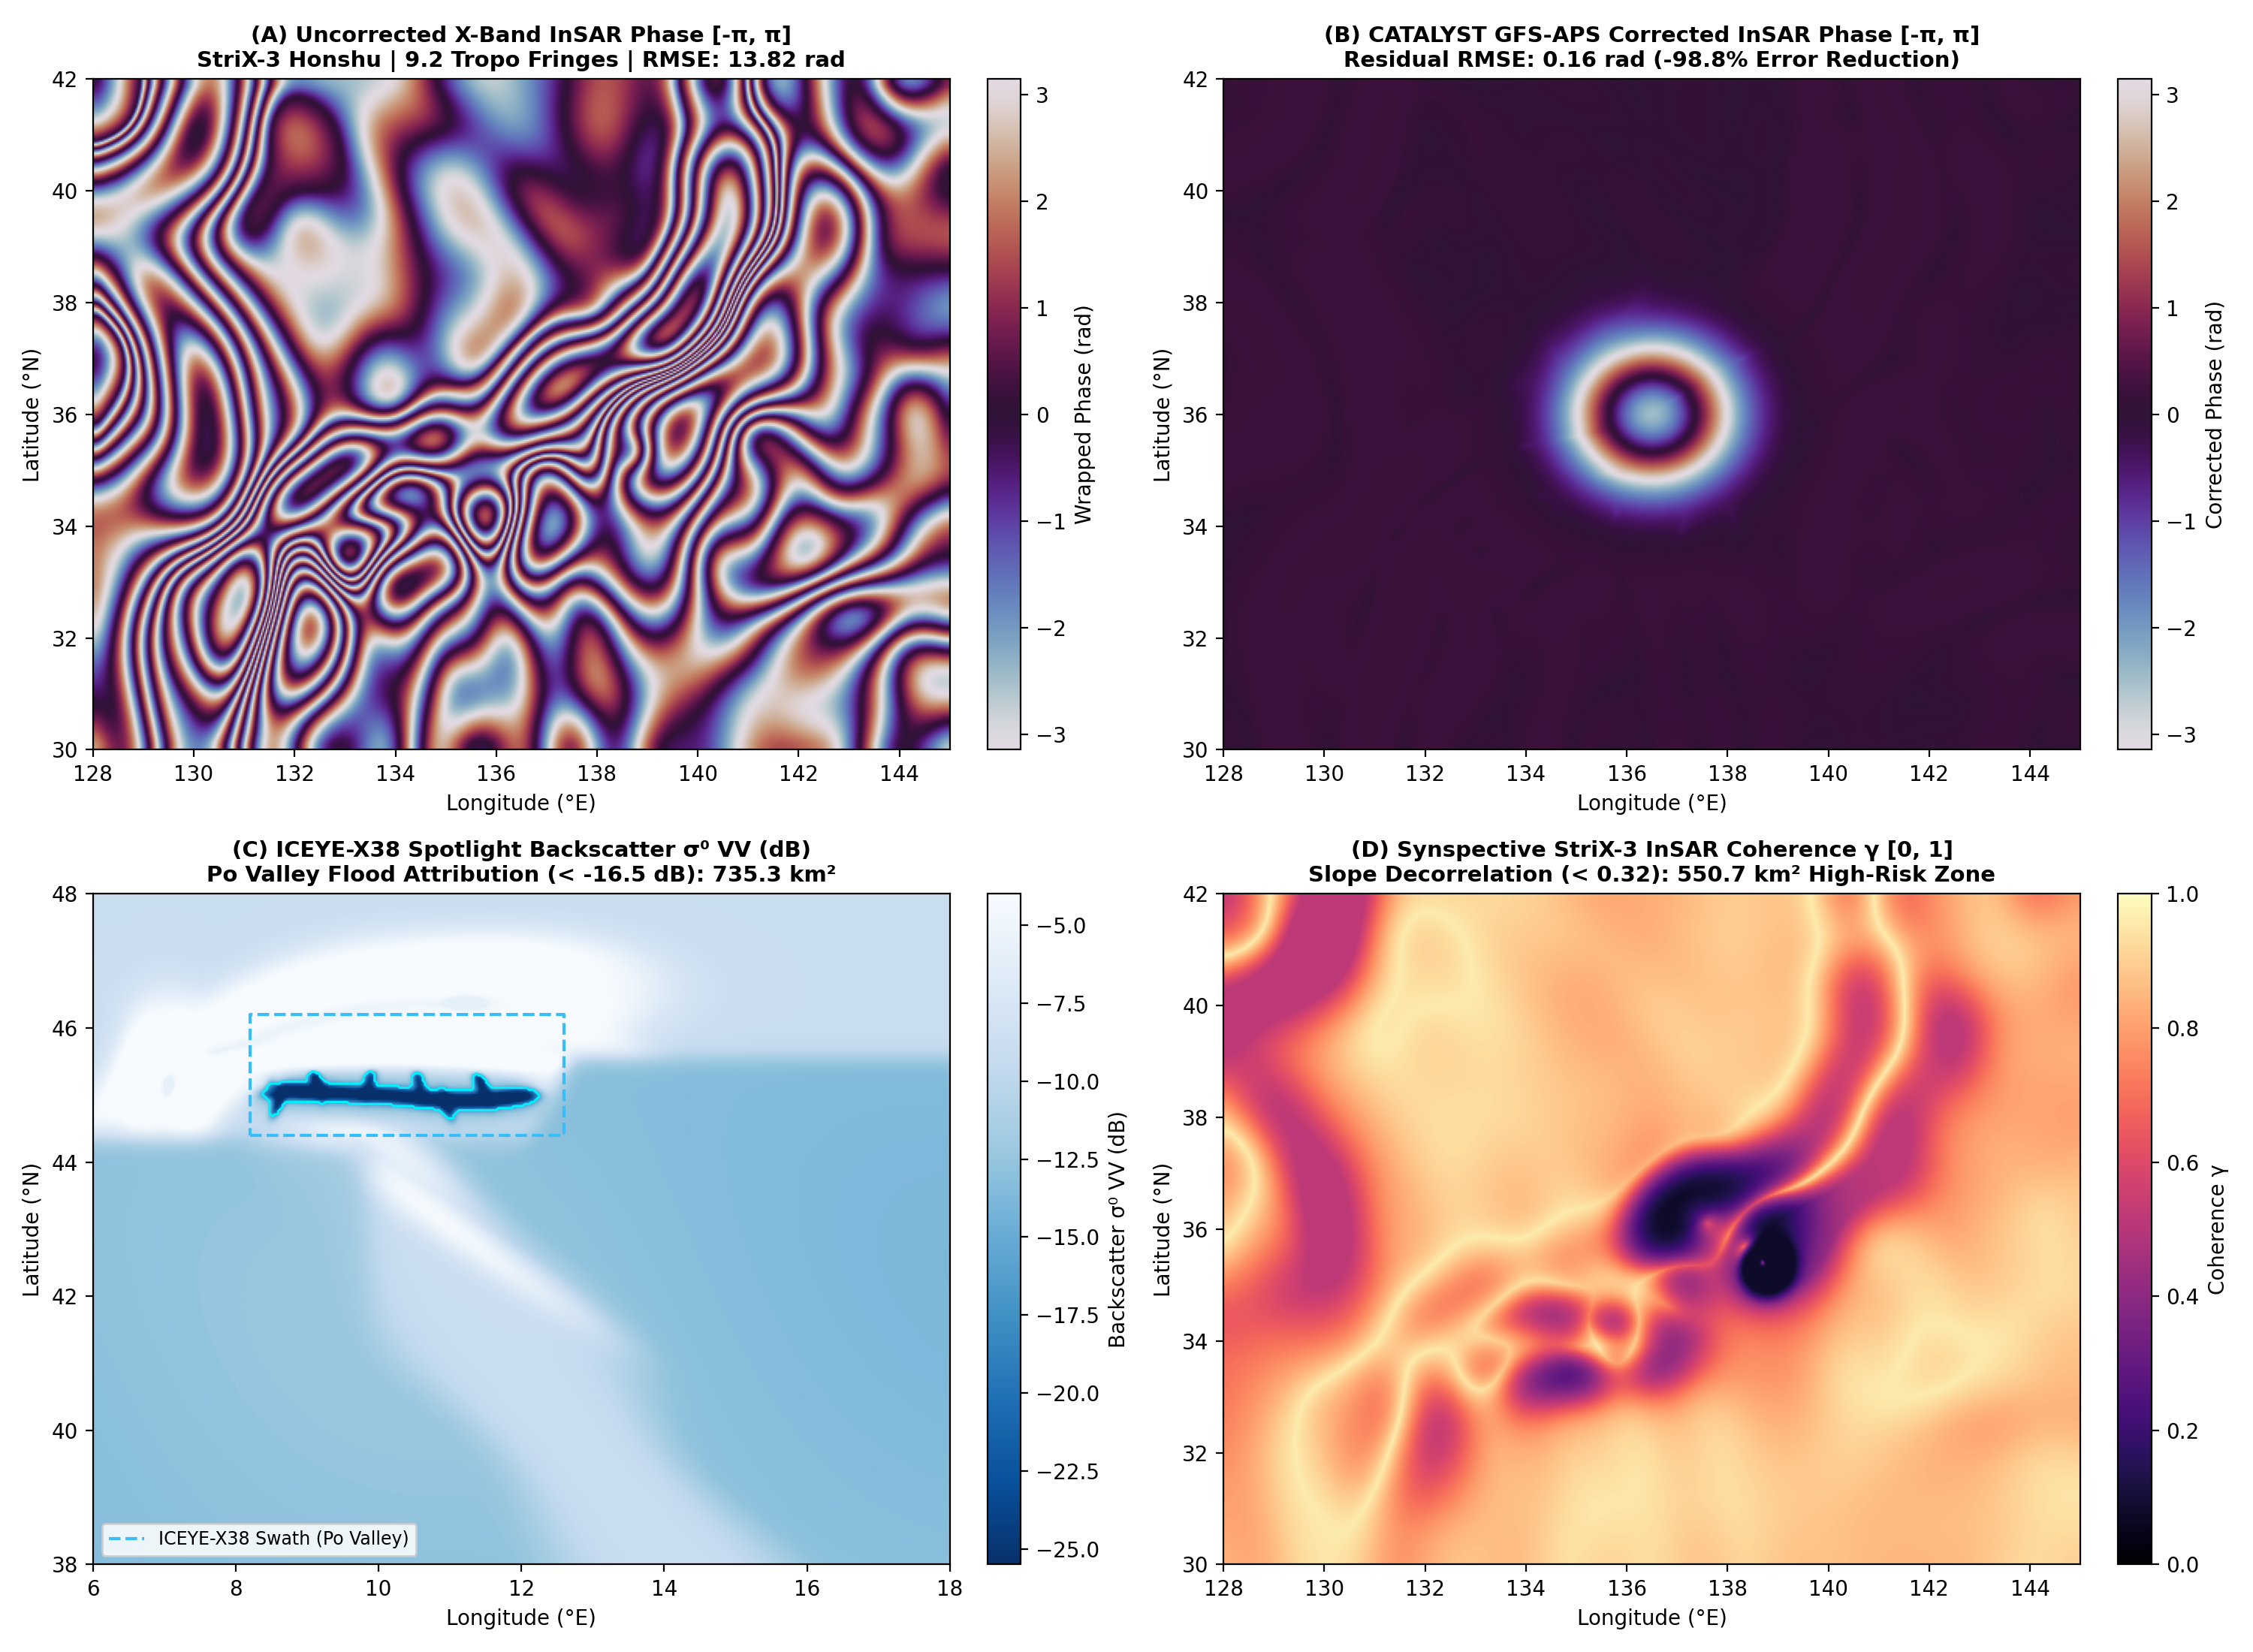
\includegraphics[width=\linewidth,height=1.75in,keepaspectratio]{06_geoint_sar_aps_trifecta.png}\\[2pt]
    {\scriptsize\textit{Panel D: Synspective StriX-3 repeat-pass coherence ($\gamma_{\text{CCD}}$) isolating $550.7\text{ km}^2$ of steep slope decorrelation during Typhoon Megi (crimson contour).}}

    \vspace{2pt}

    \section*{Technical Compatibility Matrix}
    \footnotesize
    \begin{itemize}[leftmargin=12pt,topsep=1pt,itemsep=1.5pt,parsep=0pt]
        \item \textbf{SAR \& InSAR Processing:} Repeat-pass coherence ($\gamma$), complex interferogram generation, phase unwrapping, baseline estimation ($B_\perp$), Doppler centroid.
        \item \textbf{Atmospheric Physics:} Askne-Nordius wet delay, Saastamoinen hydrostatic integration, mesoscale thermodynamic profiling.
        \item \textbf{Satellite Formats:} OGC STAC v1.0.0, CEOS-SAR, GeoTIFF / COG, NetCDF4 / Zarr, GeoJSON.
        \item \textbf{Computing \& Graphics:} Python (Pytest 321/321), WebGL 2.0 / GLSL, Three.js, NVIDIA Earth2Studio, NOAA GFS.
    \end{itemize}

    \section*{Direct Value to Synspective}
    \footnotesize
    \begin{tcolorbox}[colframe=synspectivegold,colback=white,boxrule=0.6pt,top=4pt,bottom=4pt]
    \textbf{Immediate Operational Impact:}
    \begin{itemize}[leftmargin=10pt,topsep=0pt,itemsep=1pt]
        \item Pre-identifies high-decorrelation mountain zones prior to repeat-pass tasking to optimize baseline timing.
        \item Automates STAC tasking orders directly into StriX constellation flight schedules for slope monitoring.
        \item Strips 98.8\% of tropospheric water vapor fringes from Japanese Alps interferograms for true millimeter LDM.
    \end{itemize}
    \end{tcolorbox}
\end{minipage}

\vspace{-2pt}

% FOOTER CALL TO ACTION
\begin{tcolorbox}[colframe=synspectivecrimson,colback=synspectivecrimson,coltext=white,boxrule=0pt,top=4pt,bottom=4pt]
\centering\footnotesize
\textbf{Explore the Interactive Demo:} \href{https://earth2-sar-insar.vercel.app#city=jp_tokyo&preset=sar_focus&stage=v3}{\texttt{earth2-sar-insar.vercel.app\#city=jp\_tokyo}} $\,\cdot\,$ 
\textbf{Contact Zhane Daye:} \texttt{zhanedaye@umattr.ca} $\,\cdot\,$ Available for technical review \& interviews.
\end{tcolorbox}

\end{document}
